\documentclass{article}

\usepackage{graphicx}
\usepackage{pdfpages}
\usepackage{amsmath}
\usepackage{amsfonts}
\usepackage{amssymb}
\usepackage{centernot}
\usepackage{verbatim}
\usepackage{graphicx}
\usepackage[colorlinks]{hyperref}
\usepackage{caption}
\usepackage{subcaption}
\usepackage{titlesec}
\usepackage{scrextend}
\usepackage{titlepic}
\usepackage{float}
\usepackage{wrapfig}
\usepackage{lscape}
\usepackage{rotating}
\usepackage{epstopdf}
\usepackage{pdflscape}
 \usepackage{placeins}
 \usepackage{enumitem}
\usepackage[margin=1.2in]{geometry}
\usepackage{authblk}
\usepackage{caption}

\graphicspath{{./Figures/state-figures/} {../../Figures/state-figures/} }

\title{\textbf{Rasica Network - Technical White Paper (DRAFT - V2)}}
\date{\today}

\author[1]{Darren Oliveiro-Priestnall\thanks{darren@ourfamily.io}}
\author[2]{Joseph Kearney\thanks{joseph.kearney@rasica.io}}
\affil[1]{Rasica Foundation}


\begin{document}


\includepdf [fitpaper=true] {Figures/cover-image}

\maketitle

\abstract

The Web3 movement has become a war cry for a new and better web. With the rise in popularity in consensus protocols, where users demand more control over the finances, we are now demanding more privacy, more security and more control over our data. Web3 is the idea that the same stateful protocols that are revolutionising the financial industry can also revolutionise the much-broken web. The Rasica Network aims to be a full stack solution for developers and business to build feature rich applications for the decentralized web.

\begin{center}
\vspace{50mm}
\textbf{This document is a work in progress and is subject to change.}
\end{center}

\newpage

{
  \hypersetup{linkcolor=black}
  \tableofcontents
}
\newpage

%%%%%%%%%%%%%%%%%%%%%%%%%%%%%%%%%%%

\section*{Introduction}

With the creation of Bitcoin \cite{nakamoto2008bitcoin}, we witnessed the opening of Pandora's box in terms of financial ingenuity, self-sovereignty and a shift of power from the financial elite to the people. Since the 1980's people like David Chaum have theorised about the ideas of distributed consensus-based protocols \cite{chaum1979computer}. Although a technical and social breakthrough, Bitcoin now comparatively is like sending money via cheques in terms of the raw throughput and functionality. \\

With the creation of Ethereum \cite{wood2014ethereum}, we witnessed the opening of Pandora's box for a second time. We were introduced to the concept of the world state and distributed computing which until its creation had only been theorized by people like Nick Szabo 20 years ago. The idea of decentralised finance and peer-based crowdfunding further challenged the grasp of the financial world. At this time new societal concepts such as Web3 were introduced. \\

Consensus-based protocols like blockchains introduced a method for each participant in a network to hold and transfer state in a digitally native format, applying stateful protocols to the traditionally stateless protocols that power the web, gives the web a native mechanism to authoritatively say who owns what, and who has permissions to do an action. \\

As groundbreaking a technology Etheruem is, it has some major problems in terms of scalability of feature-rich functionality. More generally with the current Web3 paradigm, trying to build decentralised applications often forces developers to adopt multiple protocols, multiple native tokens, and multiple technology stacks in return for simplistic functionality compared to our stateless ancestor protocols. \\

Our approach for building Rasica was to solve these core issues, and to:

\begin{itemize}
\item Build a true Byzantine fault-tolerant consensus that becomes increasing scalable, decentralised and secure at scale.
\item Provide a feature-rich full-stack solution to developers who want to embrace the web3 ethos.
\item Rethink the economic incentives around blockchain systems, to be fairer to all participants.
\end{itemize}


\begin{comment}
NB - To be moved to the DFS section?

Rasica solves this problem through the integration of a Distributed File System (DFS). This enables much more control for peers on the network in terms of what elements of the ledger they hold. This means that lightweight nodes can run with only a subset of the network data. Furthermore, large data files can be securely held on the ledger without causing issues for other nodes due to bloating.


\end{comment}

%%%%%%%%%%%%%%%%%%%%%%%%%%%%%%%%%%
\newpage
\section{Rasica Consensus Mechanism}

Distributed networks have no single point of trust to determine the validity of transactions, so consistency must be ensured by other methods. Typically this requires a majority of the network's participants to agree on a particular update of the ledger and the changes to account balances held on the ledger. Blockchain technologies generally employ Proof-of-Work (PoW) and occasionally Proof-of-Stake (PoS) mechanisms in order to gain consensus across a network. PoW originates from hashcash \cite{back2002hashcash}, which was designed as a prevention mechanism for email spam. This idea was then developed for the bitcoin blockchain, it required miners to perform a computationally hard problem in order for them to expend energy and there by resources. This dissuades mining nodes from acting maliciously, as both the transactions they have added as well as the work they have performed can be verified. If their work is poor then the block they are trying to append to the blockchain will be rejected \textit{i.e.} will not be considered the longest chain. This technique for consensus is Byzantine fault tolerant and can not be understated as the critical factor that has allowed blockchain technologies to grow. However, this has two critical flaws, firstly the amount of expended and wasted energy is extraordinary especially on large networks where the potential rewards are large. Secondly there has been a general trend towards centralisation at scale, as mining pools hold increase their share of the network power (and thereby the networks rewards). Other networks employ a small amount of trusted nodes that ensure the validity of transactions, but this is also highly centralised and almost as fallible as the single point of failure systems that DLTs endeavors to avoid. \\


Rasica integrates a newly designed consensus mechanism, based on Probabilistic Byzantine Fault Tolerance (PBFT). For the test-net a Proof-of-Authority (PoA) version of the consensus mechanism will be employed. While this PoA will be highly similar to the final consensus mechanism validation will be restricted to trusted user nodes. Rasica gains consensus through a collaborative mechanism by voting rather than through a competitive process. The consensus for Rasica test-net can therefore be more accurately described as a PoA voting mechanism. For each ledger cycle a worker nodes are selected from a group of trusted authorities, the nodes become the producers for a cycle or number of cycles. The producer nodes perform work in the form of compiling and validating transactions thereby extracting a ledger state change for that cycle. \\

The protocol is split into four distinct phases:

\begin{itemize}

\item Construction Phase - Producer nodes that have been selected create what they believe to be the correct update of the ledger. They then distribute this proposed ledger update in the form of a hash digest.
\item Campaigning Phase - Producer nodes designate and declare what they propose to be the ledger state update as determined by the values collected from other producer nodes in the producer pool.
\item Voting Phase - Producer nodes vote for what they believe to be the most popular ledger state update as determined by the producer pool according to the candidates for the most popular update from the other producer nodes.
\item Synchronisation Phase - The producers who have computed the correct ledger update can broadcast this update to the rest of the network.

\end{itemize}

This section is based on the work set out in \cite{Rasicaresearch}, where the original research into the creation of a new consensus mechanism is laid out. The various parameters and thresholds mentioned in this chapter and their impact on the levels of security and confidence in the successful production of a ledger state update are discussed in the following paper \cite{Rasicaresearch2}.


\subsection{Producer Node Selection}

\input{tex-files/consensus/producer-node-selection}


\subsection{Notation} 

For the sake of clarity, here is a dictionary of the variables used in the proceeding description of the consensus mechanism:

\begin{itemize}

\item $p$ - A single producer that has been selected randomly to perform work for the network for a given cycle.
\item $P$ - The pool of producers who have been selected through the producer selection mechanism for the particular cycle being described. It is made up of a set of producers $p$.z
\item $T$ - The mempool of any given producer $p$. It contains a group of transactions that will be used in the update for a given cycle.
\item $t$ - A single transaction that is found within the mempool $T$.
\item $u$ - The local ledger state update generated by a single producer node. This is what that particular node believes to be the correct update for the given cycle.
\item $\sigma$ - A pseudorandomly generated number, used as a salt.
\item $d$ - A hash tree containing all the signatures extracted from the transactions in $T$.
\item $H$ - A hash of each list $E$ combined with the salt $\sigma$.
\item $L$ - Alphanumerically ordered list of the pairs $E,H$, sorted according to $H$.
\item $G$ - The list of proposed updates $u$ that producer $p$ collects from other nodes in producer pool $P$. This is used to determine the most popular update.
\item $\#\mathcal{L}$ - The bloom filter of producers from a particular producers' set $G$ that sent the most popular ledger state update.
\item $L_{final}$ - A producers list of compensation entries \textit{i.e.} who a producer believes did the correct work for the network and thereby should be rewarded. This is created from all the combined $\#\mathcal{L}$ received. 
\item $\#\mathcal{L}_{(final)}$ - The bloom filter of producers a specific producer found in $L_{final}$.
\item $LSU$ - Ledger State Update. This is the final ledger state update proposed by a producer node. It consists of the list of transactions used to create the update, the bloom filter or producers who produced the correct partial ledger state update and the users peer ID.

\end{itemize}


\subsection{Construction Phase}

The first phase of the Rasica consensus algorithm is the Construction Phase. In this phase, the producer node who was selected $p$ calculate their proposed ledger state update. This is done by aggregating and validating all transactions that have occurred, these transactions are ordered and producers will know the target number of well formed transactions to be included in the update. These transactions, assuming their validity, are represented by the list of digital signatures extracted the transactions, from which they can create a hash of the update. This hash digest represents what they believe to be the correct update and is broadcast to the other producer nodes for that cycle. Assuming the collision free nature of hash functions, the only mechanism for multiple producer nodes to have the same local ledger state update is for both of them to use the same set of transactions. \\

$p$ follows the following protocol. The construction phase begins with producer $p$ selecting the set of $n$ transactions that are to be integrated into the next ledger update. This $n$ transactions is determined by the network meaning that it is uniform for all producers and can be considered the difficulty of the block generation. This difficulty will decrease at times of low transaction throughput and increase at times of higher demand from the network. This also means that all selected producers know how many valid transactions they should attempt to add to a ledger update. The set of transactions $T$ selected by $p$ to process is made up of a set of transactions $t$. These transaction are used to create $p$'s local ledger state update $u$. \\

This set of transactions will be ordered as and when they a received by a producer through the following process:

\begin{itemize} 
\item A hash of each transaction is created using the salt $\sigma$ which is created utilizing a pseudo-random number generator using the previous ledger state update.
\begin{center}
$H = \mathcal{H}[t~||~\sigma]$
\end{center}
\item This creates a pair ($t,H$).
\item The list of transactions $t$ are sorted alphanumerically according to $H$.
\end{itemize}

Once the threshold according to the required number of transactions has been met $p$ creates a hash tree $d$. This is to store the signatures that are extracted from each transaction in $T$ and is used as an excerpt of the ledger update. 

\begin{enumerate}


\item $d$ will be ordered equivalently to the list of selected transactions i.e. each $d$ will map in order to a corresponding transaction $t$ from $T$. 

\item The producer $p$ then extracts the transaction fee value from each transaction in $T$ to create $v$ which is the total sum of all transaction fees.

\item The local ledger state update $u$ for producer $p$ can then be calculated. This is done by concatenating (denoted by $||$) the hash tree $d$ with the producer $p$'s peer ID denoted by PId and a hash digest is created as:

\begin{center}
$u = \mathcal{H}(d~||~PId)$
\end{center}

This summary of transactions $u$ is then concatenated with $p$'s $PId$ to create:

\begin{center}
$h = u ~||~PId$
\end{center}

\item $p$ is then broadcasts $h$ as a message to the other producers.
\end{enumerate}


Producer $p$ also collects other producers' partial ledger update values. At most they will collect $P-1$ values. Optimally every producer in $P$ will receive the same set of transactions, so for every $p$ in $P$ they will have the same partial ledger update $u$. However this is unlikely due to all transactions not being received by a small group of nodes, however because each producer node knows how many . Equally they may not hold $G$ where $G = h_1,...,h_P$, meaning they may not receive a proposed update from all candidates.



\subsection{Campaigning Phase}

The second phase of the consensus mechanism is where the producer $p$ generates and proposes a candidate, which it calculates to be the most popular ledger state update. \\


Beginning this phase producer $p$ is constructing a set of proposed ledger updates $G$ that it is receiving from other producer nodes. $p$ must first reach the threshold $G_{min}$, this is the minimum number of messages $h$ that $p$ has observed that are considered acceptable for calculating an educated vote. It must the attempt to decode each of the $h_i$ values within $G$. If $p$ has not created the same $h$ as another producers $h_i$, then the received $h_i$ will not be deducible due to hash functions being irreversible. These indecipherable $h_i$ should be be placed in one group while and $h$ values that can be deciphered by: 

\begin{center} 
$h_i = \mathcal{H}(d~||~PId_i)$
\end{center} 

therefore:

\begin{center} 
$d_i == d$
\end{center} 

If this is satisfied, then it is provable that this $h_i$ from another producer used the same set of extracted signatures retrieved and thereby the same set of transactions was used. These two producers have proposed the same update. \\

This continues for all the $h_i$ values in $G$, leaving two distinct subsets of votes. Those that can be decoded and those that can not. If $p$ found the majority then the number in the subset that could be decoded should be greater that that of the size of the subset that could not. Furthermore, the number in this subset should reach a minimum threshold which is defined as:

\begin{center} 
$G_{threshold}(99.999\%) = \left( 0.5 + 4.22\sqrt{\frac{G^{dec}(G-G^{dec})}{G}}\right) \times G$
\end{center} 

Where $G$ is the total amount of votes seen, and $G^{dec}$ is the set of values that $p$ was capable of decoding. \\

If these two criteria are not met then it is assumed that the producer $p$ has failed to select the correct set of transactions and thereby has failed the consensus process. Meanwhile if these criteria have been met then the producer knows that consensus has been achieved with a subset of other successful producers. \\

If these thresholds are met $p$ then:
\begin{enumerate}
\item $p$ creates a list $\mathcal{L}$. To this list $p$ appends the $PId$ of any producer that $p$ correctly decoded the $h_i$ value. $p$ should append their own $PId$.
\item From the list $\mathcal{L}$, $p$ creates a bloom filter $\#(\mathcal{L})$. Each element of the list  $\mathcal{L}$ is added to the bloom filter. 
\item Producer $p$ then creates their candidate for the ledger update $c$ which is calculated as $c = h^{maj}~||~\#(\mathcal{L})~||~Id$
\item Producer $p$ will then broadcast their preferred update $c$ to the other producers.
\end{enumerate}

At the end of the campaigning phase the producer $p$ should broadcast three elements (under the assumption that they found themselves to be in the majority). These elements are $h^{maj}$, which in reality will be the same as the $h$ value they broadcast in the construction phase, the bloom filter $\#(\mathcal{L})$ which represents all the other producers that $p$ found to have produced the majority update and their PId. \\




\subsection{Voting Phase}

The third phase of the ledger cycle is the Voting phase. In this phase, the producer $p$ collects the $c$ values broadcast by the other producers. By this stage of the consensus algorithm, the only producers that remain should be those that have $h^{maj}$. These recieved $c$ values are incorporated into a set $C$. This set $C$ is used by the producers to determine the complete list of producers that gave the correct update and thereby those that should be rewarded for their contribution. $C_{min}$ is the minimum number of retrieved votes that a producer can have in order to give a valid final update, thereby the producer $p$ continues collecting broadcast votes $c$ until $C \geq C_{min}$. \\


Upon retrieving enough $c$ values from other producers to meet the threshold $C_{min}$, $p$ must again attempt to decode the $u^{maj}$ values contained within its set $C$. This is done as in the campaigning phase. The amount of decoded values must meet the threshold determined by:  

\begin{center} 
$C_{threshold}(99.999\%) = \left( 0.5 + 4.22\sqrt{\frac{C^{dec}(C-C^{dec})}{C}}\right) \times C$
\end{center} 

Where $C^{dec}$ is the number of values that $p$ was capable of decoding. If this threshold is met then it can be assumed that with a 99.999\% certainty that a majority of the $C$ values collected by $p$ were in fact the correct update. In reality this number should be significantly higher if not 100\% due to only the producers who hold the correct update having reached this stage of the consensus algorithm. \\

Upon confirming that $p$ is in the majority, they can now begin to produce the final list of producers that created the correct ledger state update. They, take the $C^{dec}$ subset and extract the bloom filters attached to that set. $p$ also retrieves the list of producers for that specific cycle from the DAO. For each element in the list of producers their membership is checked in each of the bloom filters in $C^{dec}$. If an element from that list appears in more that half of the bloom filters that element is added to a new list $\mathcal{L}_{final}$, upon checking all the elements from the list of producers against the retrieved bloom filters a new bloom filter is created $\#(\mathcal{L}_{final})$ containing all elements determined to have been present in more than half of the bloom filters. 

\subsection{Synchronisation Phase}

The Synchronisation Phase allows those nodes that have produced the correct ledger update to then pass this update onto the rest of the network, thereby integrating the changes held within upon the overall state of the ledger. Rasicas DFS is the mechanism for distribution of the newly formed ledger update, thereby two distinct \\

At this stage a producer $p$ who during the consensus phase managed to produce the majority update can now pass along the correct ledger update. \\

Each $p$ that found themselves to be within the majority broadcast their ledger update to the network. This takes the form: 

\begin{center} 
$LSU = \#(\mathcal{L}_{final})~||~T~||~PId$
\end{center} 

Meaning that contained within the final ledger state are three elements, the bloom filter containing all the users that a producer $p$ found to have passed on the correct ledger state updates the list of transactions $T$ that were incorporated into this ledger update, and their PId in order to verify authenticity of the update. From the LSU a CID is created that relates to the updates location on the DFS. \\

This combined with the information recorded in the transactions in the RANDAO provides users with the information required to determine which users from the pool of producers $P$ that were selected from this cycle were. \\

The producer then pins this update to the DFS, adding their name to the hash table. If they are the first to do so they also create the CID for this update. The producer can the broadcast this CID to the network, declaring that a new delta has been created. Other peers on the network can access the update and request the update from one of the producers that holds the update.

\begin{comment}

During the synchronisation phase $p$ executes the following steps:

\begin{enumerate}

\item Producer $p$ selects from the producer votes $V$ which received the most popular unique $V$. The number of most popular votes received is defined as $V_{max}$. This $V_{max}$ value must exceed a specified threshold $V_{thresh}$. So $V_{max} \geq V_{thresh}$. 

\item $p$ creates a list $\mathcal{L}_{final}(vote)$. To $\mathcal{L}_{final}(vote)$ the producer $p$ appends the identifier of any producer that their given $V == V_{max}$ \textit{i.e.} they voted among the majority. Furthermore that producer must appear in at least half the $\mathcal{L}(vote)$ lists found in the $V$ values $p$ collected from other producers. 

\item If the producer $p$ also created the correct ledger state update $LSU$ then they can write it to the DFS with the content address CID \cite{ADD LINK TO CID OBJ}.

\item Producer $p$ then creates the final producer output that can be declared to the network. This output is:
\begin{center}
\fbox{$\mathbf{o} = CID~||~\#(\mathcal{L}_{final}(vote))~||~Id$}
\label{eq:Hj}
\end{center}


The producer then broadcasts $\mathbf{o}$ to the network.
\end{enumerate}
\end{comment}
\begin{comment}

\subsubsection{Ledger state synchronisation across the network}



THIS PART NEEDS CHECKING AS THIS RELATES TO NETWORK SYNC

During the time period [$t_{s}, t_s + \Delta t_{cycle}$], user nodes collect $\{o_k\}_{\forall k \in P}$ producer outputs broadcast by the producers.
By extracting the identifier $Id_k$ embedded in any collected output $o_k$, a user node can easily compile a list of producer identifiers having broadcast the same second hash value $\mathcal{H}(\Delta L_n)$ (concatenated with the same list $\mathcal{L}_{n}(vote)$). Upon receiving $x > P/2$ identical addresses $\{\mathcal{A}_k = \mathcal{A}_n\}_{k \in x}$, the user nodes can read the common address content ($\Delta L_n$) from DFS. Using $\Delta L_n$ a user node can safely synchronise their local copy of the ledger and write it to their DFS if not already done. The balance of accounts stored on the ledger are updated and the producers effectively collect their rewards.\\


Worker nodes also store the list $\mathcal{L}_{n}(vote)$ embedded in each $o_k$ output. If selected to be a producer for the next cycle $\mathcal{C}_{n+1}$, a worker can use it to generate the reward allocated to the producers who correctly voted for the accurate ledger state update during the ledger cycle $\mathcal{C}_{n}$.\\

\begin{verbatim}
pragma solidity ^0.5.11;
contract RANDAO is Ownable
{
    int deltaHeight;
    int cycleVotes;
    int targetThreshold;
    
    struct Delta {
        bytes32 deltaHash;
    }
    struct Guest {
        address guestAddress;
        uint guestId;
    }
    struct validator {
        uint validatorId;
        bytes32 commitment;
        address validatorAddress;
    }
    address[] public stakers;
    bytes32[] public candidateDeltas;
    mapping(bytes32 => bool) commitments;
    mapping(address => Delta) public cycleVotes;    
    mapping(address => validator) public stakersMapping;
    event NodeStake(address guest);
    
    constructor
    (
        int deltaHeight
    )
    public
    {
        deltaHeight = deltaHeight;
    }
    function stakeEntry(bytes32 commitment) public payable
    {
        address _senderAddress = _msgSender();
        require(msg.value == 21 Kat, "you need more Kats to stake");
        stakersMapping[_senderAddress].guestId = stakers.push(_senderAddress) - 1;
        // generate PRNG logic here
        emit NodeStake(_senderAddress);
    }
    function voteDelta(bytes32 favouriteDelta) public payable
    {
        address _senderAddress = _msgSender();
        if(stakers[stakersMapping[_senderAddress].guestId] == _senderAddress)
        {
            if (cycleThreshold < targetThreshold)
            {
                cycleVotes[_senderAddress] = candidateDeltas.push(favouriteDelta);
            }
        }
    }
}
\end{verbatim}

\end{comment}




\subsection{Bloom Filters in Further Detail}

One key issue posed from the consensus mechanism described in \cite{TWP} is the propagation and distribution of information across producers and eventually across the entire network. This is particularly an issue for the distribution of the list of producers   that a specific producer considers to have created the correct ledger state update. With larger producer pool which are necessary for security consideration, large lists of information are impractical for distribution. When it it is considered the every PID is 32Bytes long, for a group of 1000 producers lists would reach 32KBytes if the raw lists of producers are distributed. While compression can be used, what is gained in size of the elements is lost in time for compression and decompression of the lists. This is especially true when it is considered that every producer could potentially have to decompress 999 lists from a pool of 1000 producers. Furthermore using a User Datagram Protocol (UDP) as used in Rasica, the potential for lost information on elements of that size is high. Therefore a more compact and efficient method is required. Bloom filters \\

Bloom filters are data structures that allow proof of membership of a set. They work is such a way that they can never provide a false negative i.e. showing that an element is in fact in the bloom filter as false. They can however show false positives meaning that an element that is not in the bloom filter can in fact come back true. Bloom filters are simple byte arrays of a specified length. Upon initialisation all bits within the byte array are set to 0. For each element to be added to the bloom filter it is hashed a defined number of times and the corresponding bit for the hash is flipped to a 1. For example for a small bit array \verb'0bx0000' and element \verb'Hello' is hashed to give the digest \verb'04' then the $4^{th}$ bit would be flipped so the bloom filter would become \verb'0bx1000'. This works on a modulo point, so if the digest was \verb'05' then the first bit would be flipped giving the bloom filter \verb'0bx0001'. For each element added to the bloom filter multiple hashes are created and added to the bloom filter, for example if 3 hashing functions are used 3 bits in total will be flipped in the bloom filter and these 3 flipped bits will represent the element. \\

Bloom filters are made up of four key variables, these are:

\begin{itemize} 
\item $m$ - The size of the bloom filter in bits.  
\item $n$ - The number of elements to be added to the bloom filter. 
\item $k$ - The number of hashing functions that are performed on each element added to the bloom filter. 
\item $p$ - Probability of a false positive occurring for an element within the bloom filter. 
\end{itemize} 

The size of a bloom filter can be defined by: 

\begin{center} 
$m = -(n \times log(p)) \div (log(2)^2)$
\end{center} 

The optimum hash count of a bloom filter can be defined by:

\begin{center} 
$k = (m \div n) \times log(2)$
\end{center} 

The false positive rate for a bloom filter is: 

\begin{center} 
$p = (1 - e^{-kn \div m})^k$
\end{center} 

The number of elements added to the bloom filter is uniform across all producers as this must be set to the total number of producers for one cycle. Each of these variables can be changed in order to form a bloom filter for whatever accuracy, size or amount of producers it is required.\\

The reason for choosing a bloom filter over directly transferring the lists is for size considerations. Distributing a list containing 100 or a 1000 elements will be extremely cumbersome due to the size. While a bloom filter for 1000 elements would be approximately 1.4kBytes in size. Furthermore, due to the goal of the list creation is to efficiently deduce the members of the worker pool that created the correct delta and that bloom filters are an efficient method for membership validation the use of bloom filters lends itself to the Rasica consensus algorithm. 

\subsection{Statistics}

Using the script in \cite{python} we can determine the probability of failure for any one particular node. Probability of failure is defined as the probability of any one node failing to hold a complete bloom filter of all producers who successfully produced the correct ledger state update. The process for a producer is such that, they produce a bloom filter of all producer they retrieved correct proposed ledger state updates at the beginning of the campaigning phase. This bloom filter is then passed of to  all other producers. However, due to natural inefficiencies it is unlikely all producers will receive all of the proposed updates therefore, the correct list must be constructed from all the received bloom filters. It is this created list for each producer that we will test. We analyse two variables, firstly is the message propagation ratio, this is the percentage of messages that we assume each producer recieves from the rest of the network, i.e. at a message propagation ratio of 0.75, for a producer pool of 100, each producer would receive randomly 75 other producers bloom filters. The second variable we will be testing is the size of the producer pool. 


%%%%%%%%%%%%%%%%%%%%%%%%%%%%%%%%%%%
\newpage
\section{Distributed File System}

Running a full node on many blockchains requires a significant amount of disk space, for example the Ethereum blockchain size has exceeded 1Tb \cite{EthBloat} and continues to grow. Rasica solves this problem through the integration of a Distributed File System (DFS). This enables much more control for peers on the network what elements of the ledger that they hold. This means lightweight nodes can be deployed. Furthermore, large data files can be securely held on the ledger without causing issues for other nodes due to bloating. \\

Rasica integrates its own Distributed File System (DFS) \cite{DFS} based on the InterPlanetary File System (IPFS) protocol \cite{benet2014ipfs}. DFS, as the name suggests, is a peer to peer file system, where the files contained within are distributed across and accessible to a range of peers on a network. This file system will have no down time nor any single point of failure (baring complete downtime of the internet), meaning that it is persistent in a way that other, centralised file storage technologies are not. IPFS is a peer to peer protocol that allows storage of files across many nodes, this is done by giving each item stored a unique identifier and providing a lookup mechanism pairing nodes that hold a item of data with the items unique identifier. Any duplicates are removed across the network, this is done as two identical files will always receive the same identifier. Using this identifier a file can be looked up on the network and retrieved from those nodes that are holding the file. Using this IPFS protocol as the basis for the DFS on Rasica means that the information that is transacted on the network does not need to be stored `on chain', meaning that there is a separation of DLT and stored data, allowing nodes to pick and choose what data they hold so any information not relevant to a particular node is not held. \\ % Why is DFS different than IPFS? Why not use IPFS directly? What is different in your implementation?

On the Rasica network every node is required to hold a DFS module. While all nodes will not hold all of the information stored on the DFS, they will be able to query and retrieve any information on the network. Furthermore, nodes will have the ability to query the existence of a file rather than being forced to download the file in order to check its existence. Nodes are required to hold the DFS module as it is used to store all information about the network.  Some of the data secured on the DFS is the critical data that is used to sync the state of new nodes joining the network. This means that this data must be accessible at all times. Therefore, if a node wishes to check any single transaction on the network or even the overall state of the ledger itself it will have to be in sync with the network, which is done through the DFS.  \\ % What information will the nodes be forced to have? Does every node have its own garbage collection implemented? How will they query the existence of files - is it content addressed? How is it content addressed?

Integrating DFS allows the Rasica network to remain lean as nodes on the network can choose to store only the data that they choose to hold. Furthermore, it allows the storage of many rich file types in a distributed manner, meaning that they are always accessible with no down time guaranteed (excluding the potential case of the internet being down). This is further under the assumption that at least one node on the network holds the data. This also requires some nodes on the network to hold the file, if all nodes remove or unpin a file then that data will no longer be accessible to the network and must be re-added by a node. It is likely that if no nodes on the network require the file and therefore it is removed from the network that the file was redundent form use.\\ % As long as nodes continue to pin that information, sure. Shouldn't we mention that? Also, you can't ensure the uptime of the internet as a whole, so downtime is still possible.



In this section is a description of the IPFS platform that Rasica uses, and then how Rasica integrates this into its ecosystem. Furthermore how the marketplace go the buying and selling of storage will operate. 

\subsection{IPFS}

The InterPlanetary File System forms the basis of the Rasica DFS. IPFS is a collection of protocols which specify how nodes are supposed to operate within the network, and various multilingual implementations of these protocols. As it is distributed, there is no one central entity that holds and controls the flow of information and most importantly who has access. Across the IPFS network nodes hold as little or as much data as the wish with multiple copies of the data being held across many unrelated nodes. This means that there is no single point of failure in the network. An attempted attack on the IPFS would require a majority of nodes to be taken offline to prevent access to the files held on the network.   \\

IPFS uses a bittorrent style seeding system. Meaning that the holder of any particular file that is online will seed the file to other peers that request the file. This means that the more peers on the network the more efficiently files can be distributed. IPFS user have the ability to `pin' files meaning that those files are stored and secured by the peer. IPFS works in such a way that the more popular \textit{i.e.} the more peers that have pinned the file, the more easily accessible that file will be.   \\

In traditional computer file systems, files are indexed, referenced, and accessed through their location: for instance, \verb`~/Documents/file.md` would refer to a Markdown file inside a "Documents" folder inside the home directory of a user on UNIX systems. However, on a distributed system, there can be no global state that could be used for addressing content. Instead of location-addressing, IPFS and other distributed systems use content-addressing. The CID also means that all files stored on IPFS are immutable i.e. can not be edited as changing anything contained within the file means that that CID for that file will now be changed. Through linkage of these files it means that a version history of files can be created. \\

In a content-addressed system, every file on the system is given a unique, deterministic content identifier (CID) by hashing the content. Hashing works by deterministically using the contents of the file as the input for a standard encryption algorithm. Changing the contents of a file would change the hash of the file. This CID can then be used to index, reference, and access the file directly, regardless of where it is. Advantageously, through content addressing, a malicious entity would not be able to send a user a false file in the place of the one that they have requested. This is due to the difficulty of reversing a hashing function. The CID associated with a file means that the file is not duplicated on the network. For example if Alice uploads file $x$ it is stored on IPFS, other users can then download and hold the file, if then Bob uploads the same file $x$ then because the CID for both files would be the same the duplication would not take place as the file is already held on the file system.  \\

Once a file has a CID associated with it, a distributed hash table (DHT) can be formed. DHTs are key-value stores, where the key is the CID of the relevant file, and the value is an array containing all of the user IDs of any peer which holds the file. The DHT is used by peers looking for a file to find the peers that it can retrieve it from. Once a user has retrieved the file from another peer in the DHT, it can also then be added as a peer that holds the file. \\

IPFS integrates Merkle Directed Acyclic Graphs (Merkle DAGs). Merkle DAGs are abstract trees which result when multiple CIDs are used as the input for another hashing algorithm, resulting in chains where entire hierarchies of files can be referenced using a single CID. Any change to any constituent file at the bottom of the tree (the leaf nodes) percolates up to the next hash, and the next, causing the CID for the entire tree to change. Merkle DAG's are used compared to traditional Merkle trees as the allow a flow or direction of information to be established. Thereby allowing an order for the reading of the files to be set. 


\subsection{Integrating the DFS}

Every node running on the Rasica network must also be running the DFS module. This allows them on the most basic level to access the current state of the ledger and the validate previous updates to the ledger thereby allowing them to sync with the current ledger state. This is required as it is necessary for the all nodes on the network at the very least to know the current state of the ledger in order to send transactions. \\

The primary difference between the native IPFS protocol and the implementation utilised on Rasica is how the peer IDs are created.  While on the IPFS protocol the identifier for nodes is selected randomly, on Rasica the nodes on the network will each have their own individual peer identifier\cite{BytesExtentions} made up of:

\begin{itemize}
\item IP address
\item Port number
\item Public key
\end{itemize}

% Can't you create your own ID in IPFS? Why not just mandate IPFS interoperability with your own peer names? Are you forking the rest of IPFS's functionality?

This allows user to be able to identify who on the network is holding specific files as each peer identifier for a node will be unique. This means that a peer on the network will have a clear target for where they can retrieve given information, furthermore it means that nodes claiming to hold specific files and information are accountable for being able to distribute these files. Through the use of Rasica peer identifiers within the DHTs peers can make informed decisions on who they retrieve files from, for example if a node has been marked as malicious due to actions within the network, they will also not be trusted within the DFS.


\subsection{The Marketplace}

\textbf{WIP} \\

The Rasica network allows nodes to be rewarded for storing data added to the DFS by other nodes on the network. These may include large files or complex data sets. The reason for payment for holding of data is to provide incentive for peers on the network to store data for others. The market place works as a method of pairing nodes who wish to store data with those that have excess space they wish to sell. By incentivising the process of storage of data on the ledger it can be ensured that when uploaded a file is persistent and accessible at all times. \\

One key issue for this marketplace is ensuring that those nodes that are claiming to store a particular element of data are in fact storing it. Furthermore, it needs to be ensured that these nodes are online are respond to requests for the data in a timely manor. In some situations this data may need to be checked with a high frequency, for others it may be a long term storage solution. It must also be ensured that a particular storage node does not already hold the information that it is being requested to store, as this will lead to the node being paid twice for storing the same item. \\

Rasica network utilises the Proof of Replication (PoR) and Proof of Space Time (PoST) mechanisms laid out by Filecoin \cite{benet2018filecoin}. Furthermore, through the use of the 0x protocol \cite{warren20170x} so all storage purchase requests can be settled on chain.  \\

PoR allows a storage node to prove to another peer on the network that a file given to it has been replicated and is unique. This means that this individual piece of data has been copied by the storage node and is held in a unique compartment of physical storage, \textit{i.e.} that this is the first time this node has been asked to store this file and they are not getting paid twice for storing one file. This is important as the node storing the data on the DFS may (and in all likelihood will) want to store the data across multiple nodes to prevent a single point of failure. PoR prevents the storage node accepting multiple bids from the node storing their file on the DFS and taking multiple rewards for it. \\

PoST is an audit process for the storage nodes. It allows the creation of a challenge, the response to this challenge from a storage node allows it to demonstrate that it has stored the data required of it and furthermore that it is consistently storing the data without the need to repeatedly require it to present the data. 
%%%%%%%%%%%%%%%%%%%%%%%%%%%%%%%%%%%
\newpage
\section{Global Ledger State}
The global ledger state is the current state of all the accounts in the Rasica Network. The state contains a key and value pair for every account. The `key' is the account address and the `value' contains account details such as the current account balance, and the number of previous transactions created from that account. A newly created account will only become part of the ledger state once it receives a transfer of Kats.
\\
\\
The global ledger state is not stored in the delta, instead a copy of the ledger state is stored by all participating nodes and updated each ledger cycle.

\subsection{Account State}
Due to Rasica Network’s extension of the Ethereum Virtual Machine into the RVM, the account information stored in the Rasica account state is similar to an Ethereum account. Smart contracts and ordinary accounts use the same account structure, however some fields contain default values except in the case of a smart contract account. \\

The variables stored in the account state are:

\begin{description}[labelwidth=2cm, leftmargin=!]
\item [Balance] The number of Mol \cite{KATUnit} owned by the account.
\item [Commitment] The private balance, represented by a Pedersen Commitment.
\item [Nonce] A number which is incremented when either public or private transactions are made from the account in order to prevent double spend attacks.
\item [StorageRoot] A hash representing the data stored by a smart contract.
\item [CodeHash] A hash representing the RVM code defining how the smart contract will operate.
\end{description}
\vspace{0.75em}
In the Rasica Network the the balance is stored directly in the state, rather than being derived from the transaction history as in Bitcoin. This has a number of advantages. New transactions can be validated more efficiently because it is faster to check that an account has sufficient funds. In addition, being able to store data state makes smart contracts much easier to design.

\subsection{Ledger Storage}

The global ledger state is stored locally by each node in a key value pair database. Any performant database such as RocksDb can be used to store the state data, however the data must be organised using a structure called a sparse Merkle tree. This structure allows the entire data state to be represented by a single hash, known as the root hash. Any changes to the data would result in a completely different root hash, therefore it can be used by nodes to verify that their dataset is the same as that of other nodes. Consequently, a node using an alternative storage organisation would be unable to interact with the network due to an inability to calculate the same root hash.\\

The sparse Merkle tree data structure allows for:

\begin{enumerate}
\item Persistent storage of the current and previous states of the ledger.
\item Efficient provision of proof that queried data exists, or importantly, does not exist in the ledger.\end{enumerate}

In addition to storing the global ledger state in a sparse Merkle tree, the smart contract RVM code and smart contract data are also stored using this data structure. This allows the root hash of both these data sets to be stored in the \textbf{storageRoot} and \textbf{codeHash} fields in the account state.  The use of the SMT for storing these data sets allows honest nodes to recognise and reject information that has been altered outside of the ledger cycle by malicious parties. \\

\subsubsection{Merkle Tree}

Each item of data being stored is represented as a leaf of the Merkle tree. The data in neighbouring leaves is hashed and concatenated and this value is used for the node one level above in the tree. Each node is stored in the database with its lookup key being the hash of its value. The nodes are themselves combined until a single hash has been obtained. This is the root hash and its value depends on every bit of data stored in the tree.\\

\begin{figure}[h]
  \centering
  \captionsetup{format=hang, font=footnotesize}
  \caption{A binary Merkle tree.}
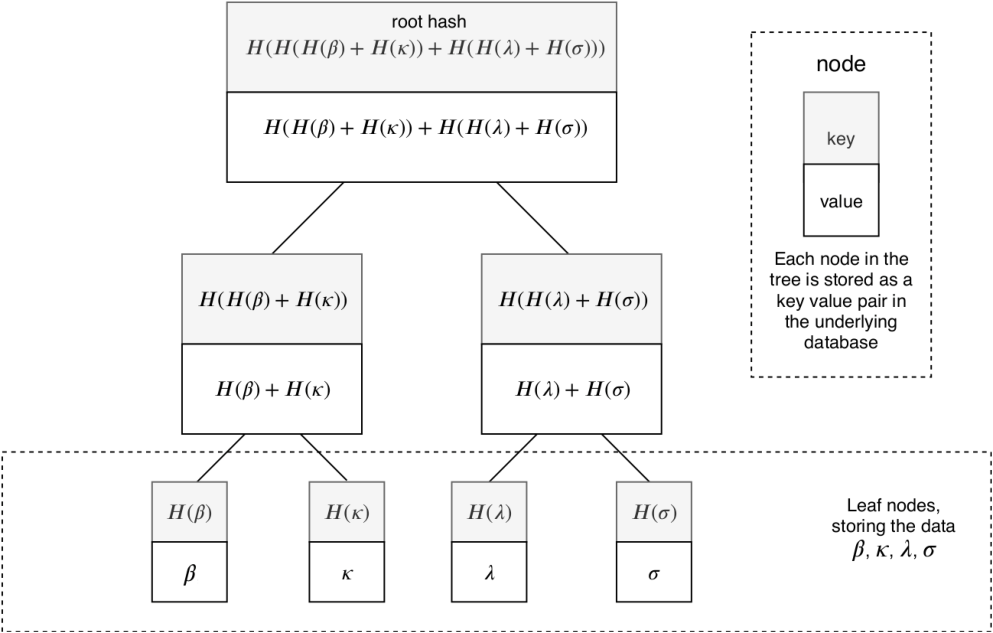
\includegraphics[scale=0.8]{merkle-tree}
\end{figure}

A binary tree is one in which the nodes can have only two children. Note that not all Merkle trees are binary trees. For example the nodes in a Modified Merkle Patricia tree can have up to 16 children.\\

When a data entry changes, every node above it in the tree must be recalculated. The hash of the data held by a node is used as its key in the database, therefore every recalculated node will constitute a new entry in the underlying database, rather than an existing entry that needs to be updated. This means that previous states of the tree are not overwritten, and all old data can be accessed using previous root hashes.\\

\subsubsection{Merkle Proof}

A client with knowledge of the current root hash of the state tree does not need to retrieve the complete set of data to verify the inclusion of a specific entry. Knowledge of each sibling hash along the path down to the entry being authenticated is sufficient to reconstruct the root hash. A client who is able to reconstruct the root hash from this data can be confident that the entry is contained in the data set. For example, in the diagram above, the inclusion of entry $\beta$ can be verified with just $\beta$, $H(\kappa)$, and $H(\lambda)+H(\sigma)$. \\

Though it is simple to prove inclusion of an item using a Merkle tree, proving that a particular item is \emph{not} included can be harder. This is because the item could exist at any of the leaf nodes.\\

\subsubsection{Sparse Merkle Tree}

The Sparse Merkle tree is a binary tree. The position of an entry in the sparse merkle tree is determined by its hash. For the ledger state, we use the hash of the account address to determine the index of the leaf node to hold the account data. This account index is used to determine the path from the root hash to the data entry, telling us which branch to follow as we progress down the tree. The account index is not equivalent to a key in the underlying database.\\

In a sparse tree a default value is used for leaves that do not yet contain data.\\

\begin{figure}[h]
  \centering
  \captionsetup{format=hang, font=footnotesize}
 \caption{A sparse Merkle tree, containing a single entry. The default values are represented by $\phi$.}
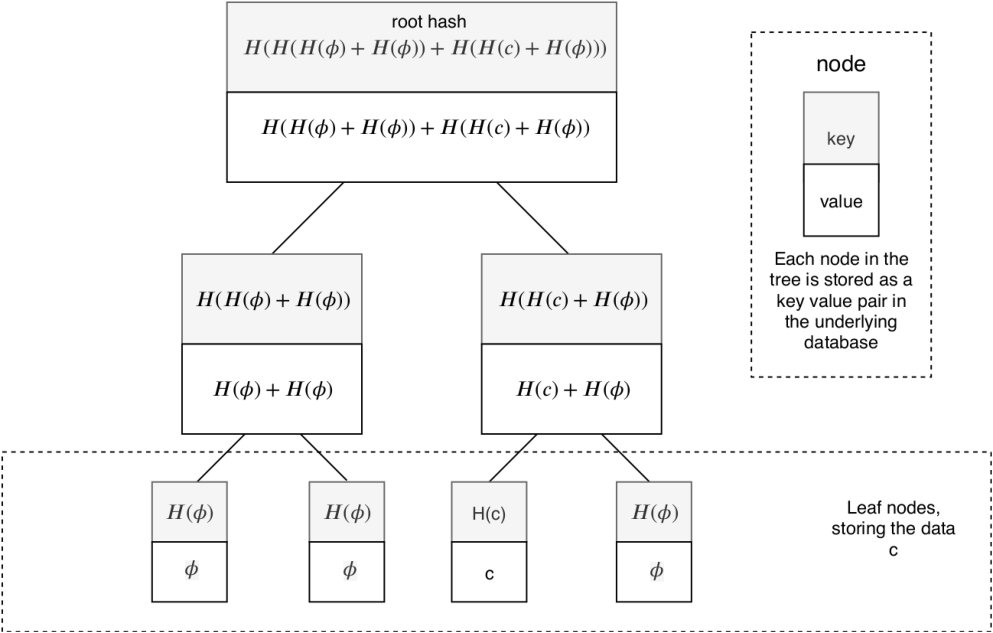
\includegraphics[scale=0.8]{sparse-merkle-tree}
\end{figure}

Since a data entry in a sparse Merkle tree can only exist in a specific location, proofs of non-inclusion are easy to provide; the proof that a key is not included in the tree is simply a proof that the value for the key is default.\\

A naive implementation would require a tree with a leaf for each possible index. Using the hash of the address as the index gives $2^{256}$ possible indices, too many to generate a full tree. However, non default entries will be uncommon compared to default entries; most of the nodes will therefore have default values that can be determined based on the height of the node. These values do not need to be stored more than once. For a branch containing only one non default entry, the entry can be stored in topmost node for that branch, providing further storage savings.\\
 
\subsubsection{Choice of Sparse Merkle Tree over the Modified Merkle Patricia Tree}

In a Patricia tree, each node can contain up to 16 children. As the sparse Merkle tree is a binary tree, it is simpler both to implement and to traverse the path to a leaf.  \\

For the Patricia tree, the Merkle proof is composed of all the nodes in the path. Since each node has 16 children the amount of data is larger and not as straightforward to verify as in a binary tree. Using a sparse Merkle tree gives us Merkle proofs which are small and easy to use.\\



\subsection{Updating the State}
The current state of the ledger can always be obtained by applying the relevant deltas to a previous state. This process is deterministic such that applying the correct updates will always create an identical new state tree. Where data is unchanged the previous entries do not need to change in order to be included in the new state.\\

The merkle tree data structure has the additional advantage that as we apply each delta we do not overwrite information from previous ledger states. This means that the ledger history can be easily queried. \\

\subsection{Retrieving the Current Ledger State}

When a new node (one that has no knowledge of the current ledger state) joins the network it must synchronise with the other nodes on the network. This means that it must get the current ledger state. While the Rasica network does not require knowledge of every single transaction performed on the network since the genesis block, a node can not simply download the current ledger state. This would be prone to error or potential malicious activity. Therefore a node must recreate the current ledger state from the genesis block. \\

New nodes on the network have knowledge of the hard coded genesis state i.e. the initial state of the network at the beginning of its life. The new node then proceeds to request the current delta height from its connected peers. From these responses the producer will select the group of nodes that provide the highest value. The new node will then request the CID's for the ledger state updates in chunks. Currently producers will request 20 at a time, this protocol takes place as follows: \\

\begin{itemize} 

\item New node requests current delta height from other connected peers. 
\item Other connected peers reply and a majority of height $x$ is found. 
\item New node initially requests a chunk of CID's from the genesis block to a high to 20 blocks so $0,\cdots,19$.
\item Upon receiving these CID's, the node compares the first element of the list i.e. the CID for state 0 to the known value for this element i.e. the genesis state. 
\item If this matches up then the corresponding files on the DFS are downloaded for the CID's given. 
\item Each of these downloaded ledger state updates are applied in order to the base state. 
\item Concurrently the next chunk of CID's are requested i.e.  $19,\cdots,28$.
\item As delta 19 is now the known value these values are compared. 
\item This process repeats until all ledger state updates have been applied to the genesis state. 
\item The outcome being that the node is now in sync. 

\end{itemize} 



%%%%%%%%%%%%%%%%%%%%%%%%%%%%%%%%%%%
\newpage
\section{RVM}

\input{tex-files/RVM/RVM-intro}

\subsection{From the SVM}

\input{tex-files/RVM/SVM}

\subsection{To the RVM}

\input{tex-files/RVM/RVM}

%%%%%%%%%%%%%%%%%%%%%%%%%%%%%%%%%%%


%%%%%%%%%%%%%%%%%%%%%%%%%%%%%%%%%%%
\newpage
\section*{Conclusion}

Rasica employs a combination of existing technologies and novel techniques in order to create an infrastructure, that allows powerful storage and manipulation of data on the network, while also ensuring fair and easy accessibility for users. This allows a network that becomes more decentralised, secure and scalable as the network size grows. Furthermore it provides an environment withing which files can be stored effectively and securely while also providing the tools for complex business logic to be created.  \\

Further information on Rasica and its applications can be found at: \\
\begin{center}
Rasica website - \url{https://www.Rasicanet.org/}\\
Rasica GitHub - \url{https://www.github.com/Rasica-network}\\
\end{center}


\bibliography{Rasica-technical-whitepaper}
\bibliographystyle{ieeetr}

\end{document}